\documentclass[twoside,twocolumn]{article}

\usepackage{blindtext} 
\usepackage{graphicx}
\usepackage[sc]{mathpazo} 
\usepackage[T1]{fontenc} 
\linespread{1.05} 
\usepackage{microtype} 


\usepackage[english]{babel} 


\usepackage[hmarginratio=1:1,top=32mm,columnsep=20pt]{geometry} 
\usepackage[hang, small,labelfont=bf,up,textfont=it,up]{caption} 
\usepackage{booktabs} 


\usepackage{lettrine} 


\usepackage{enumitem} 
\setlist[itemize]{noitemsep} 


\usepackage{abstract} 
\renewcommand{\abstractnamefont}{\normalfont\bfseries} 
\renewcommand{\abstracttextfont}{\normalfont\small\itshape} 


\usepackage{titlesec} 
\renewcommand\thesection{\Roman{section}} % 
\renewcommand\thesubsection{\roman{subsection}} 
\titleformat{\section}[block]{\large\scshape\centering}{\thesection.}{1em}{} 
\titleformat{\subsection}[block]{\large}{\thesubsection.}{1em}{} 


\usepackage{fancyhdr} 
\pagestyle{fancy} 
\fancyhead{} 
\fancyfoot{} 
\fancyhead[C]{Titulo $\bullet$ Junio 2019 $\bullet$ } 
\fancyfoot[RO,LE]{\thepage} 


\usepackage{titling} 


\usepackage{hyperref} 


%----------------------------------------------------------------------------------------
%	TILULOS
%----------------------------------------------------------------------------------------


\setlength{\droptitle}{-4\baselineskip} 

\pretitle{\begin{center}\Huge\bfseries} 
\posttitle{\end{center}} 
\title{Business Intelligence and Business Analytics} 
\author{José Edilberto, Pastor Mendoza, Franklin Carlos, Huichi Contreras, Sigfredo, Aponte Roldán, \\
Jesus Enrique, Sandoval blas. }
\date{\today} 
\renewcommand{\maketitlehookd}{
\begin{abstract}
\noindent 
Business Intelligence BI is a tool, below different kind organizations, supports
decisions making processes, based in an exact and accurate information;
guarantying the production of the needed knowledge that lets to choose the most
appropiate option for the company success. The investigation begins with the BI
definition and applications; by addition shows definitions and relevant BI
investigations tools, like Data Warehouse, Olap, Balance Scorecard and Data
Mining.
\end{abstract}
\begin{abstract}
\noindent 

Treva es un sistema enfocado en los formularios de satisfacion del cliente en donde el propietario podra generar formularios y enviar cada cierto tiempo a sus empleado o interesados para que puedan llenarlo segun
las opciones que cuenta el formulario, a partir de esos datos podemos al propietario dar estadisticas en la cual puede verificar que opciones escogieron los clientes o empleados, y aparte de ello podemos analizar los datos
para dar recomendaciones o proyecciones estimadas de areas especificas.

\end{abstract}
}

%----------------------------------------------------------------------------------------

\begin{document}

% Print the title
\maketitle

%----------------------------------------------------------------------------------------
%	INTRODUCCION
%----------------------------------------------------------------------------------------

\section{Introduccion}
\lettrine[nindent=0em,lines=3]{A}ctualmente en el Perú las pequeñas y medianas empresas producen al mercado peruano ingresos y empleo, la gran cantidad de informacion que manejan es debido al alto numero de operaciones que realizan a diario, por lo tanto se necesita una forma de controlar los datos como las opiniones de los clientes y de esta forma conseguir retroalimentacion instantanea para las empresas. Asimismo tener la informacion en reportes descriptivos para la visualizacion se ha hecho parte importante de los sistemas de hoy para tomar desiciones acertadas y utiles para las empresasl.\\ \\

\section{Titulo}
El sistema se identifica con el titulo de treva.\\ \\

\section{Autores}
\begin{itemize}
\item José Edilberto, Pastor Mendoza.
\item Franklin Carlos, Huichi Contreras.
\item Sigfredo, Aponte Roldán.
\item Jesus Enrique, Sandoval blas.
\end{itemize}
\section{Planteamiento del problema}
Actualmente en el Perú las pequeñas y medianas empresas producen al mercado peruano ingresos y empleo, la gran cantidad de informacion que manejan es debido al alto numero de operaciones que realizan a diario.\\ \\

\subsection{Problema}
Actualmente en el Perú las pequeñas y medianas empresas producen al mercado peruano ingresos y empleo, la gran cantidad de informacion que manejan es debido al alto numero de operaciones que realizan a diario.\\ \\

\subsection{Justificacion}
Actualmente en el Perú las pequeñas y medianas empresas producen al mercado peruano ingresos y empleo, la gran cantidad de informacion que manejan es debido al alto numero de operaciones que realizan a diario.\\ \\

\subsection{Alcance}
Para el alcance de este proyecto nesecitaremos de clientes que quieran realizar sus formularios de satisfaccion y ofrecerles todas las herramientas nesecarias para que lo hagan de manera eficaz. Alcanzado la meta podremos generar los dashboards que ayude al cliente a ver los resultados entre otros indicadores.


\section{Objetivos}
Actualmente en el Perú las pequeñas y medianas empresas producen al mercado peruano ingresos y empleo, la gran cantidad de informacion que manejan es debido al alto numero de operaciones que realizan a diario.\\ \\

\subsection{General}
Actualmente en el Perú las pequeñas y medianas empresas producen al mercado peruano ingresos y empleo, la gran cantidad de informacion que manejan es debido al alto numero de operaciones que realizan a diario.\\ \\

\subsection{Especificos}
Actualmente en el Perú las pequeñas y medianas empresas producen al mercado peruano ingresos y empleo, la gran cantidad de informacion que manejan es debido al alto numero de operaciones que realizan a diario.\\ \\

\section{Referentes teoricos}
Actualmente en el Perú las pequeñas y medianas empresas producen al mercado peruano ingresos y empleo, la gran cantidad de informacion que manejan es debido al alto numero de operaciones que realizan a diario.\\ \\

\section{Desarrollo de la propuesta}
Actualmente en el Perú las pequeñas y medianas empresas producen al mercado peruano ingresos y empleo, la gran cantidad de informacion que manejan es debido al alto numero de operaciones que realizan a diario.\\ \\

\subsection{Tecnologia de informacion}
Actualmente en el Perú las pequeñas y medianas empresas producen al mercado peruano ingresos y empleo, la gran cantidad de informacion que manejan es debido al alto numero de operaciones que realizan a diario.\\ \\

\subsection{Metodologia, tecnicas usadas}
Actualmente en el Perú las pequeñas y medianas empresas producen al mercado peruano ingresos y empleo, la gran cantidad de informacion que manejan es debido al alto numero de operaciones que realizan a diario.\\ \\

\section{Cronograma}
\begin{figure}[htb]
	\begin{center}
		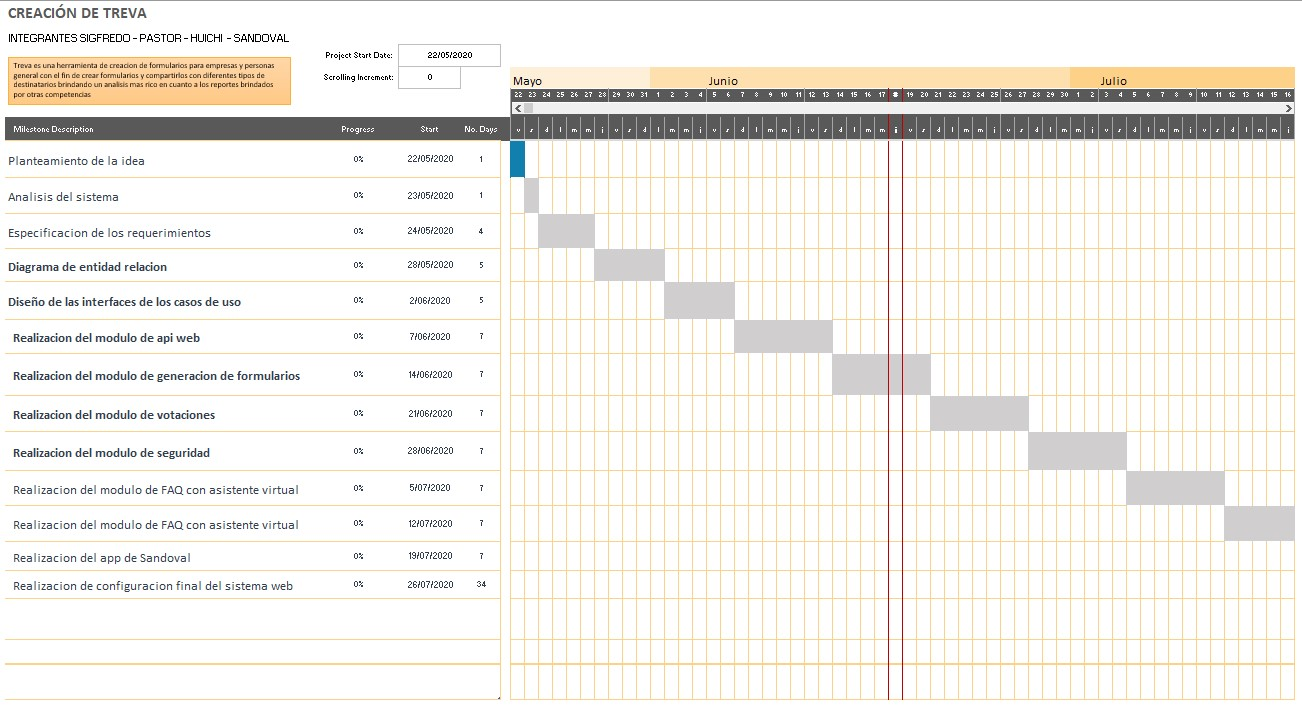
\includegraphics[width=7.5cm]{./IMAGENES/Cronograma} 
		\caption{Cronograma}
	\end{center}
\end{figure}



%----------------------------------------------------------------------------------------
%	BIBLIOGRAFIA
%----------------------------------------------------------------------------------------


\begin{thebibliography}{99} 

\bibitem[Silvia Chavez y Carmen Contreras, 2018]{}
\newblock Implementación de Business Intelligence, para el proceso de toma de decisiones del área de ventas.

\bibitem[Hans Peter Luhn 1958]{}
\newblock A Business Intelligence System

\bibitem[Alex Rayón, 2015]{Universidad de Deusto}
Conceptos básicos del Business Intelligence.

\bibitem[Jordi Conesa y Josep Curto, 2010]{}
\newblock Introduccion al Business Intelligence

\bibitem[Margaret Rouse, 2019]{}
\newblock Análisis de negocios (BA)

\bibitem[Noodle Editorial Staff, 2018]{}
\newblock Business analytics career paths

\bibitem[Josep Lluis Cano, 2007]{}
\newblock Business Intelligence: competir con información


\bibitem[Curto J., 2010]{} 
\newblock Introducción al Business Intelligence. Editorial UOC.

\bibitem[Kimball R. and Ross M., 2002]{} 
\newblock  The Data Warehouse Toolkit: The Complete Guide to Dimensional Modeling. Wiley
 
\end{thebibliography}


%----------------------------------------------------------------------------------------


\end{document}
